\section{\hotpot\ Architecture and Abstraction}
\label{sec:hotpot:design}
\label{sec:hotpot:abstraction}

We built {\em \hotpot}, a kernel-level \dsnvm\ system that %manages \dsnvm\ and
%manages distributed shared persistent memory
provides applications with direct memory load/store access to both local and remote \nvm\
and a mechanism to make in-\nvm\ data durable, consistent, and reliable.
\hotpot\ is easy to use, delivers low-latency performance, 
and provides flexible choices of data consistency, reliability, and availability levels.
This section presents the overall architecture of \hotpot\ and its abstraction to applications.

We built most of \hotpot\ as a loadable kernel module in Linux 3.11.0 
with only a few small changes to the original kernel. 
\hotpot\ has around 19K lines of code, out of which 6.4K lines are for a customized network stack (Section~\ref{sec:hotpot:network}).

\hotpot\ sits in the kernel space and manages \nvm{}s in a set of distributed nodes, or {\em \hotpot\ nodes}.
\hotpot\ provides applications with an easy-to-use, memory-based abstraction that encapsulates 
both memory and persistent data access in a transparent way.
Figure~\ref{fig-hotpot-architecture} presents \hotpot's architecture.
\hotpot\ uses a {\em Central Dispatcher (\cd)} 
to manage node membership and initialization tasks (\eg, create a dataset).
All data and metadata communication after a dataset has been created takes place between \hotpot\ nodes and does not involve the \cd.

{
\begin{figure}[th]
\begin{center}
\centerline{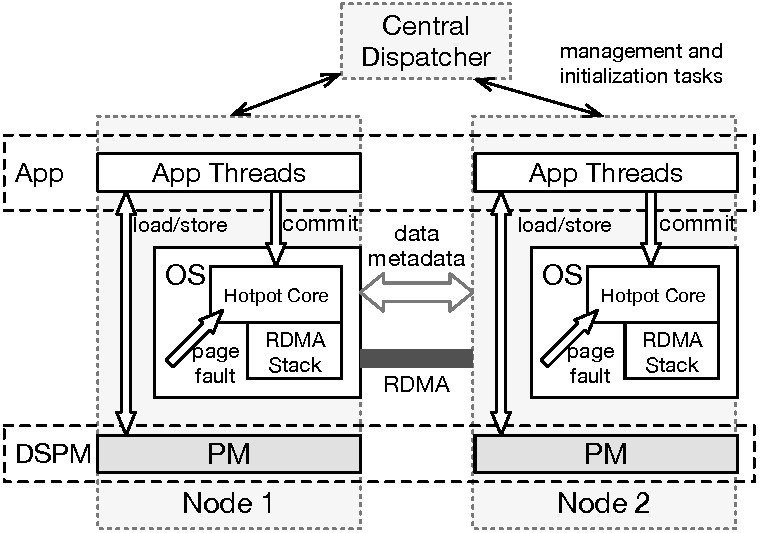
\includegraphics[width=0.4\textwidth]{Figures/architecture.pdf}}
\vspace{-0.1in}
\mycaption{fig-architecture}{\hotpot\ Architecture.}
{
%Illustration of \hotpot\ architecture. 
%\nvm{}s on the two \hotpot\ nodes form a global \dsnvm\ space.
%An application can run several application threads on each node.
}
\end{center}
\vspace{-0.1in}
\end{figure}
}


\subsection{Application Execution and Data Access Abstraction}
Most data-intensive applications are multithreaded 
and distribute their data processing work across threads~\cite{MongoDB,Gonzalez12-OSDI}.
Thus, \hotpot\ adopts a thread-based model to run applications on a set of \hotpot\ nodes.
\hotpot\ uses application threads as the unit of deployment and
lets applications decide what operations and what data accesses they want to include in each thread.
Applications specify what threads to run on each \hotpot\ node 
and \hotpot\ runs an application by starting all its threads together on all \hotpot\ nodes. 
We give users full flexibility in choosing their initial thread and workload distributions.
However, such user-chosen distributions may not be optimal, especially as workloads change over time.
To remedy this situation, 
\hotpot\ provides a mechanism to adaptively move data closer to computation based on workload behavior, 
as will be discussed in Section~\ref{sec:hotpot:migration}.


\hotpot\ provides a global virtual memory address space to each application.
Application threads running on a node can perform native memory load and store instructions using global virtual memory addresses 
to access both local and remote \nvm.
The applications do not know where their data physically is or whether a memory access is local or remote.
Internally, a virtual memory address can map to a local physical page if the page exists locally or 
generate a page fault which will be fulfilled by \hotpot\ by fetching a remote page (more in Section \ref{sec:hotpot:readwrite}). 
Figure~\ref{fig-hotpot-addressing} presents an example of \hotpot's global virtual address space.
Unlike an I/O-based interface, \hotpot's native memory interface can best exploit \nvm{}s' low-latency, DRAM-like performance, and byte addressability.

On top of the memory load/store interfaces, \hotpot\ provides a mechanism for applications to 
name their data,
APIs to make their data persistent, %: \beginxact, \commitxact, and \commit,
and helper functions for distributed thread synchronization. 
%We will discuss these three APIs in detail in Section~~\ref{sec:xact}.
Table~\ref{tbl-apis} lists \hotpot\ APIs.
We also illustrate \hotpot's programming model with a simple program in Figure~\ref{fig-code-eg}.
We will explain \hotpot's data commit semantics in Section~\ref{sec:hotpot:xact}.

{
\begin{table}[t]\normalsize
\begin{center}
\caption[\hotpot\ APIs.]{
Apart from these APIs, \hotpot\ also supports direct memory loads and stores.
}
\begin{center}
\begin{tabular} { p{1.2in} | p{2.5in} | p{1.8in} }
\normalsize API & \normalsize Explanation & \normalsize Backward \\
\hline
\hline
\open\ \ \ \ (\close) & open or create (close) a \dsnvm\ dataset & same as current \\
\hline
\mmap\ (\unmap) & map (unmap) a \dsnvm\ region in a dataset to application address space & same as current \\
%\close\ & close a \dsnvm\ dataset & same as file \close\ \\
\hline
\commit\  & commit a set of data and make $N$ persistent replicas & similar to msync \\
\hline
\acquire\  & acquire single writer permission & \\
%\fetch\ & fetch a set of committed data & \\
\hline
%\commit\ & atomically commit dirty data and make $N$ persistent replicas & same as current \\
%\hline
\barrier\ & helper function to synchronize threads on different nodes & similar to pthread barrier \\
\end{tabular}
\end{center}
\label{tbl-apis}
\end{center}
\end{table}
}
{
\begin{figure}[th]
\begin{center}
\centerline{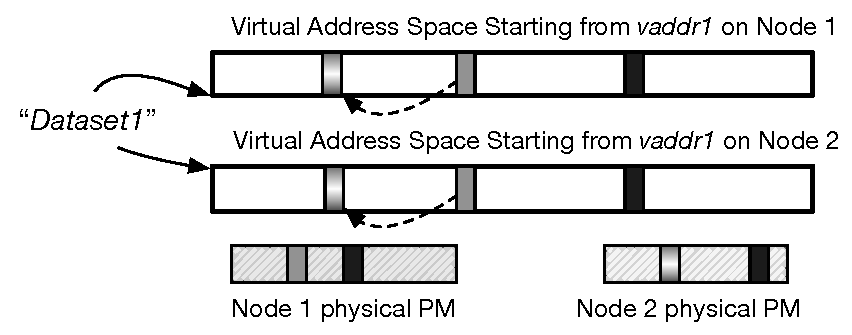
\includegraphics[width=\textwidth]{hotpot/Figures/addressing.pdf}}
\caption[\hotpot\ Addressing.]
{\hotpot\ Addressing.
\hotpot\ maps ``{\em Dataset1}'' to Node 1 and Node 2's virtual address space using the 
same base virtual addresses. The physical address mapping on each node is different.
The grey blocks in the middle are pointers that point to the blocks on the left. 
}
\label{fig-hotpot-addressing}
\end{center}
\end{figure}
}

\subsection{Persistent Naming}
\label{sec:hotpot:naming}
To be able to store persistent data and to allow applications to re-open them after closing or failures, 
\hotpot\ needs to provide a naming mechanism that can sustain power recycles and crashes. 

Many modern data-intensive applications such as in-memory databases~\cite{MongoDB} and graphs~\cite{Gonzalez14-OSDI,Gonzalez12-OSDI}
work with only one or a few big datasets that include all of an application's data 
and then manage their own fine-grained data structures within these datasets.
Thus, instead of traditional hierarchical file naming, 
we adopt a flat naming mechanism in \hotpot\ to reduce metadata management overhead. % to let applications name their persistent data in \dsnvm.

Specifically, \hotpot\ applications assign names by {\em datasets}
and can use these names to open the datasets.
A dataset is similar to the traditional file concept, 
but \hotpot\ places all datasets directly under a mounted \hotpot\ partition without any directories or hierarchies.
Since under \hotpot's targeted application usage, there will only be a few big datasets,
dataset lookup and metadata management with \hotpot's flat namespace are easy and efficient.
We use a simple (persistent) hash table internally to lookup datasets. 

The \open\ and \mmap\ APIs in Table~\ref{tbl-apis} let applications create or open a dataset with a name and 
map it into the application's virtual memory address space.
Afterwards, all data access is through native memory instructions.

{
\begin{figure}[th]
\begin{center}
\scriptsize
\lstinputlisting[
language=C
]{hotpot/code-eg.c}
\caption[Sample code using \hotpot.]{Sample code using \hotpot.}
\label{fig-code-eg}
\end{center}
\end{figure}
}


\subsection{Consistent and Persistent Pointers} 
\label{sec:hotpot:addressing}

\hotpot\ applications can use \dsnvm\ as memory and store arbitrary data structures in it. 
One resulting challenge is the management of pointers in \dsnvm.
To make it easy to build persistent applications with memory semantics, 
\hotpot\ ensures that pointers in \dsnvm\ have the same value (\ie, virtual addresses of the data that they point to) 
both across nodes and across crashes. 
Application threads on different \hotpot\ nodes can use pointers directly without pointer marshaling or unmarshaling,
even after power failure.
We call such pointers {\em globally-consistent and persistent pointers}.
Similar to NV-Heaps~\cite{Coburn11-ASPLOS}, we restrict \dsnvm\ pointers to only point to data within the same dataset. 
Our targeted type of applications which build their internal data structures within big datasets already meet this requirement.

To support globally-consistent and persistent pointers, 
\hotpot\ guarantees that the same virtual memory address is used as the starting address of a dataset across nodes and across re-opens of the dataset.
With the same base virtual address of a dataset and virtual addresses within a dataset being consecutive, 
all pointers across \hotpot\ nodes will have the same value. 

We developed a new mechanism to guarantee that the same base virtual address is used across nodes and crashes.
When an application opens a dataset for the first time, \hotpot\ uses a consensus protocol to discover the current 
available virtual address ranges on all nodes and select one for the dataset. 
Nodes that have not opened the dataset will reserve this virtual address range for possible future opening of the dataset.
Since the total amount of virtual addresses for \dsnvm\ is bound to the total size of \dsnvm\ datasets, 
\hotpot\ can always find available virtual address ranges on 64-bit platforms.
\hotpot\ records the virtual address range persistently and forces applications to use the same virtual address 
the next time it starts.
To ensure that recorded persistent virtual address ranges are always available when opening datasets, 
we change the kernel loader and virtual memory address allocator (\ie, {\it brk} implementation) to exclude 
all recorded address ranges.
